\documentclass[12pt]{report}

%-------------------------------------------------------
% THEMES, COLORS
%-------------------------------------------------------
\usepackage[top=2.5cm, bottom=3cm, left=2.5cm, right=2.5cm]{geometry}
\usepackage{amsmath,mathtools,bm,amsthm}
\usepackage{underscore}
\usepackage{xcolor}
\usepackage{graphicx}
\usepackage{algpseudocode}

%--------------------------------------------------------
% COLOR DEFINITIONS
%---------------------------------------------------------
\definecolor{amber}{rgb}{1.0, 0.49, 0.0}
\definecolor{olivedrab}{rgb}{0.42, 0.56, 0.14}
\definecolor{darkolivegreen}{rgb}{0.33, 0.42, 0.18}
\definecolor{chromeyellow}{rgb}{1.0, 0.65, 0.0}
\definecolor{beige}{rgb}{0.96, 0.96, 0.86}
\definecolor{bluegreen}{rgb}{3, 166, 155}
\definecolor{pitchblack}{rgb}{0, 0, 0}
\definecolor{lightbeige}{rgb}{255, 251, 241}
\definecolor{mediumgray}{rgb}{183, 183, 183}
\definecolor{carrotorange}{rgb}{0.93, 0.57, 0.13}
\definecolor{orange-red}{rgb}{1.0, 0.27, 0.0}
\definecolor{ferngreen}{rgb}{0.31, 0.47, 0.26}
\definecolor{darkspringgreen}{rgb}{0.09, 0.45, 0.27}
\definecolor{cocoabrown}{rgb}{0.82, 0.41, 0.12}
\definecolor{darkorange}{rgb}{1.0, 0.55, 0.0}
\definecolor{deepcarrotorange}{rgb}{0.91, 0.41, 0.17}
%---------------------------------------------------------

%-------------------------------------------------------------------------
% NEW THEME
%-------------------------------------------------------------------------
\definecolor{UBCblue}{rgb}{0.04706, 0.13725, 0.26667} % UBC Blue (primary)
\definecolor{UBCgrey}{rgb}{0.3686, 0.5255, 0.6235} % UBC Grey (secondary)

%\usepackage{helvet}
%-------------------------------------------------------
% DEFFINING AND REDEFINING COMMANDS
%-------------------------------------------------------
\newcommand\var{\texttt}
\usepackage{amssymb}
\renewcommand{\emptyset}{\varnothing}

%-----------------------------------------------------------------------------
% FONT PACKAGES
%-----------------------------------------------------------------------------

\usepackage[utf8]{inputenc}
\usepackage[english]{babel}
\usepackage{sectsty}
%\allsectionsfont{\mdseries}
%\usepackage{fontspec}
\usepackage[T1]{fontenc}
\usepackage{lmodern}
%\usepackage{charter}
%\usepackage[bitstream-charter]{mathdesign}
%\usepackage{fourier}
%-----------------------------------------------------------------------------
% FONTS TRIED
%-----------------------------------------------------------------------------
%\usepackage{ccfonts}
%\usepackage{mathpazo}
%\usepackage{newtxtext}
%\usepackage{newtxmath}
%% Times New Roman
%\setromanfont[
%BoldFont=timesbd.ttf,
%ItalicFont=timesi.ttf,
%BoldItalicFont=timesbi.ttf,
%]{times.ttf}
%% Arial
%\setsansfont[
%BoldFont=arialbd.ttf,
%ItalicFont=ariali.ttf,
%BoldItalicFont=arialbi.ttf
%]{arial.ttf}
%% Courier New
%\setmonofont[Scale=0.90,
%BoldFont=courbd.ttf,
%ItalicFont=couri.ttf,
%BoldItalicFont=courbi.ttf
%]{cour.ttf}



%-------------------------------------------------------
% INFORMATION IN THE TITLE PAGE
%-------------------------------------------------------


\newtheorem{lemma}{Lemma}[chapter]
\newtheorem{theorem}{Theorem}[chapter]
\theoremstyle{definition}
\newtheorem{definition}{Definition}[chapter]
\newtheorem{example}{Example}[chapter]
\newtheorem*{note}{Note}
\newcommand{\samplecomp}{m_{\mathcal{H}}}
\newcommand{\SampleComp}[2]{m_{\mathcal{H}}(#1, #2)}
\newcommand{\usamplecomp}[2]{m_{\mathcal{H}}^{\text{UC}}(#1, #2)}
\newcommand{\USampleComp}{m_{\mathcal{H}}^{\text{UC}}}
\newcommand{\nusamplecomp}{\ensuremath{m_{\mathcal{H}}^{\text{NUL}}}}
\newcommand{\pacerror}[1]{L_{\mathcal{D}, f}(#1)}
\newcommand{\vcdim}{\ensuremath{\text{VCdim}}}
\newcommand{\algo}{\ensuremath{\mathcal{A}}}
\newcommand{\hypclass}{\ensuremath{\mathcal{H}}}
\newcommand{\parity}[1]{\ensuremath{\mathcal{H}_{#1\text{-parity}}}}
\newcommand{\rect}[1]{\ensuremath{\mathcal{H}_{\text{rect}}^{#1}}}
\newcommand{\conj}[1]{\ensuremath{\mathcal{H}_{\text{con}}^{#1}}}
\newcommand{\mconj}[1]{\ensuremath{\mathcal{H}_{\text{mcon}}^{#1}}}
\newcommand{\zeroone}{\ensuremath{\operatorname{0-1}}}
\newcommand{\dom}{\ensuremath{\mathcal{X}}}
\newcommand{\range}{\ensuremath{\mathcal{Y}}}
\newcommand{\Nat}{\ensuremath{\mathbf{N}}}
\newcommand{\dist}{\ensuremath{\mathcal{D}}}
\newcommand{\R}{\ensuremath{\mathbf{R}}}
\newcommand{\Rone}{\ensuremath{\mathbf{R}}}
\newcommand{\Rpos}{\ensuremath{\mathbf{R}_{+}}}
\newcommand{\Rtwo}{\ensuremath{\mathbf{R}^2}}
\newcommand{\Prtwo}[2]{\mathbf{Pr}_{#1} \left \{ #2 \right \}}
\newcommand{\Prone}[1]{\mathbf{Pr} \left \{ #1 \right \}}
\newcommand{\Exptwo}[2]{\mathbf{E}_{#1} \left [ #2 \right ]}
\newcommand{\Expone}[1]{\mathbf{E} \left [ #1 \right ]}
\newcommand{\ceiling}[1]{\ensuremath{\left \lceil #1 \right \rceil}}
\newcommand{\angular}[1]{\ensuremath{\left \langle #1 \right \rangle}}
\newcommand{\floor}[1]{\ensuremath{\left \lfloor #1 \right \rfloor}}
\newcommand{\dx}{\ensuremath{\text{d}}}
\newcommand{\ind}{\ensuremath{\mathbf{1}}}
\newcommand{\Mod}[1]{\ (\mathrm{mod}\ #1)}
\newcommand{\basisvec}{\ensuremath{\mathbf{e}}}
\newcommand{\vect}[1]{\ensuremath{\mathbf{#1}}}

\DeclareMathOperator{\ERM}{ERM}
\DeclareMathOperator{\pos}{POS}
\DeclareMathOperator{\HS}{HS}
\DeclareMathOperator{\HHS}{HHS}
\DeclareMathOperator{\id}{id}
\DeclareMathOperator{\sign}{sign}

\title{Understanding Machine Learning: Exercises}

\author{Somnath Sikdar}
\date{\today}

\begin{document}
\maketitle
\tableofcontents

\chapter*{What this is About}

\addcontentsline{toc}{chapter}{\protect\numberline{}About this Document}

These notes are my attempt to understand and work out material from the
textbook \emph{Understanding Machine Learning} by Shai Shalev-Shwartz and
Shai Ben-David. 

\setcounter{chapter}{2}
\chapter{Improving the Way Neural Networks Learn}

\section{The Cross-Entropy Cost Function}

\begin{exercise}
Show that the cross-entropy function is minimized when $\sigma(z) = y$ for all inputs.
\end{exercise}
\begin{solution}
The cross-entropy function is defined as:
\[
    C = - \frac{1}{m} \sum_{i = 1}^m [y_i \ln (a_i) + (1 - y_i) \ln (1 - a_i)],
\]
where the $y_i$s are fixed and the $a_i$s are the ``variables.'' Now $\partial C / \partial a_i$
is given by:
\[
    \frac{\partial C}{\partial a_i} = \frac{1}{m} \frac{a_i - y_i}{a_i (1 - a_i)}. 
\]
At an extremum point of $C$, each component of the gradient $\nabla_a C$ will be zero. This 
happens when $a_i = y_i$ for all~$1 \leq i \leq m$. 

As a side note, the function $H(y) = - [y \ln(y) + (1 - y) \ln (1 - y)]$ for $y \in (0, 1)$ 
is called the binary entropy function and behaves as shown in Figure~\ref{fig:binary_entropy}. 
\end{solution}

\begin{figure}[ht]
\begin{center}
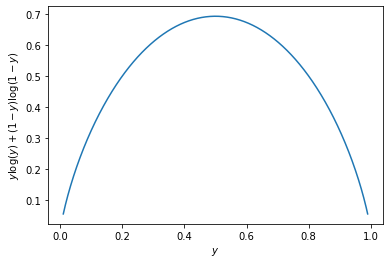
\includegraphics[scale=0.60]{entropy.png}
\end{center}
\caption{The Binary Entropy Function}
\label{fig:binary_entropy}
\end{figure}

\begin{exercise}
Partial derivatives of the cross-entropy cost function in multi-layer
networks.
\end{exercise}
\begin{solution}
The cross-entropy function for a single training example~$x$ for the last
layer~$L$ of the network is defined as:
\[
    C(x) = - \sum_j \left [ y_j \ln (a_j^L) + (1 - y_j) \ln(1 - a_j^L) \right ],
\]
where the sum is over all neurons~$j$ in layer~$L$. To recap notation,  
\[
a_j^L = \sigma(z_j^L) = \sum_k w_{j k}^L a_k^{L - 1} + b_j^L.
\]
For this training example~$x$,
\begin{align*}
    \frac{\partial C(x)}{\partial z_j^L} 
        & = - \frac{y_j}{a_j^L} \cdot \sigma' (z_j^L) + \frac{1 - y_j}{1 - a_j^L} \cdot \sigma' (z_j^L) \\
        & = \frac{-y_j + y_j a_j^L + a_j^L - y_j a_j^L}{a_j^L (1 - a_j^L)} \cdot \sigma' (z_j^L) \\
        & = a_j^L - y_j.
\end{align*}
The last equality follows since $\sigma' (z_j^L) = a_j^L (1 - a_j^L)$.

Again, for this single training example~$x$, $\partial C (x) / \partial w_{j k}^L$ 
is given by:
\begin{align*}
    \frac{\partial C (x)}{\partial w_{j k}^L} 
        & = \frac{\partial C}{\partial z_j^L} \cdot \frac{\partial z_j^L}{\partial w_{j k}^L} \\
        & = (a_j^l - y_j) \cdot a_k^{L - 1}. 
\end{align*}
For $n$ training examples, the cost function is defined as $\frac{1}{n} \sum_{x} C(x)$ and 
this derivative is: 
\[
    \frac{\partial C}{\partial w_{j k}^L} = \frac{1}{n} \sum_x a_k^{L - 1} (a_j^L - y_j).
\]
If we were to replace $C(x)$ by the usual quadratic cost $\frac{1}{2}(y_j - a_j^L)^2$, then 
the same derivative would have been:
\[
    \frac{1}{n} \sum_x a_k^{L - 1} (a_j^L - y_j) \cdot \sigma' (z_j^L).
\]
\end{solution}

\subsection{Deriving the Cross-Entropy Function}

Given a single neuron with $r$ input weights $w_1, \ldots, w_r$ and bias~$b$,
and a single input $\vect{x} = \trans{(x_1, \ldots, x_r)}$, we would like the
cost function $C$ to depend on the weights and the bias as follows:
\begin{align}
    \frac{\partial C}{\partial w_j} & = x_j (a - y) \\
    \frac{\partial C}{\partial b}   & = a - y, \label{eqn:cost_bias}
\end{align}
where $a = \sigma(\sum_{j} w_j x_j + b)$ and $y$ is the desired output 
corresponding to $\vect{x}$. 

Using the chain rule, we obtain:
\begin{align}
    \frac{\partial C}{\partial b} & = 
        \frac{\partial C}{\partial a} \cdot 
        \frac{\partial a}{\partial z} \cdot 
        \frac{\partial z}{\partial b} \nonumber \\
        & = \frac{\partial C}{\partial a} \cdot \sigma'(z) \nonumber \\ 
        & = \frac{\partial C}{\partial a} \cdot a (1 - a) \label{eqn:cross_entropy} 
\end{align}
From equations~(\ref{eqn:cost_bias} and~\ref{eqn:cross_entropy}), we obtain:
\[
    \frac{\partial C}{\partial a} = \frac{a - y}{a (1 - a)} = 
        \frac{1}{1 - a} - y \left ( \frac{1}{1 - a} + \frac{1}{a}\right ).
\]
Integrating both sides wrt~$a$, we obtain:
\[
    C = - [(1 - y) \ln (1 - a) + y \ln (a)] + \text{ a constant}.
\]

\section{Softmax}

Consider a classification problem, where labelled examples take the form 
$(\vect{x}, \vect{y})$, where $\vect{x} \in \R^m$ and $\vect{y} \in \{0, 1\}^J$ 
denotes to which of the $J$ classes $\vect{x}$ belongs to. 
In such cases, it makes sense to have the last 
layer of the neural network to have $J$ neurons with the softmax activation:
\begin{align*}
    z_j^L & = \sum_k w_{j k}^L a_{k}^{L - 1} + b_j \\
    a_j^L & = \frac{e^{z_j^L}}{ \sum_{i = 1}^J e^{z_i^L}}
\end{align*}

The cost associated with the input $(\vect{x}, \vect{y})$ where $y_r = 1$ 
is defined as the negative log-likelihood of the activation $a_{r}^L$:
\[
    C(\vect{x}, \vect{y}) = - \ln a_{r}^L.
\]

The partial derivatives $\partial C / \partial b_j^L$ and   $\partial C / \partial w_{j k}^L$
can be computed easily as follows. Depending on whether the index $j$ and the class index~$r$
are the same or not, we have two cases for each partial derivative.
\begin{align}
    \frac{\partial C}{\partial b_{r}^L} 
        & =   - \frac{1}{a_{r}^L} \cdot 
            \left [ \frac{e^{z_{r}^L}}{ \sum_{i = 1}^J e^{z_i^L}} - 
                    \left ( \frac{e^{z_{r}^L}}{ \sum_{i = 1}^J e^{z_i^L}} \right )^2 
            \right ] = - 1 + a_{r}^L \\
\frac{\partial C}{\partial b_j^L} 
      & = 
    - \frac{1}{a_{r}^L} \cdot \left [ 0 - \frac{e^{z_{r}^L} e^{z_j^L}}{ \left ( \sum_{i = 1}^J e^{z_i^L} \right )^2} 
                            \right ] = a_j^L. 
\end{align}
The first equation is when the index $r = j$ and the second when $r \neq j$. 
These two expressions can be summarized into one: 
\begin{equation}
\frac{\partial C}{\partial b_j^L} = a_{j}^L - y_j.
\end{equation}

Similarly, the partial derivative expression for  $\partial C / \partial w_{j k}^L$
can be written as:
\begin{equation}
\frac{\partial C}{\partial w_{j k}^L} = a_{k}^{L - 1} \cdot (a_{j}^L - y_j). 
\end{equation}

\begin{exercise}
Where does the ``softmax'' name come from? Consider the following variant 
of the softmax function:
\[
    a_j^L =  \frac{e^{c z_j^L}}{ \sum_{i = 1}^J e^{c z_i^L}},
\]
where $c$ is a positive constant. What is the limit of $a_j^L$ 
as $c \to \infty$?
\end{exercise}
\begin{solution}
Let $z_r^L = \max_i \{z_i^L\}$. We could then write the modified softmax
function as:
\[
    a_j^L =  \frac{e^{c (z_j^L - z_r^L)}}{ 1 + \sum_{i \neq r} e^{c (z_i^L - z_r^L)}}. 
\]
If $j = r$, then the numerator is $1$ and the denominator approaches $1$ as $c \to \infty$
and $a_j^L \to 1$. On the other hand, if $j \neq r$, the numerator $\to 0$ as $c \to \infty$;
the denominator in any case approaches~$1$ and hence~$a_j^L \to 0$. The point here is 
that $a_j^L = 1$ if $z_j^L$ is the maximum and $a_j^L = 0$ otherwise. 
\end{solution}


\chapter{Learning via Uniform Convergence}

\section*{Notes on Chapter 4}

Given any hypothesis class $\hypclass$ and a domain $Z = \dom \times Y$, let
$l$ be a loss function from $\hypclass \times Z \rightarrow \Rpos$. Finally let
$\dist$ be a distribution over the domain $Z$. The risk of a hypothesis $h \in
\hypclass$ is
\[
    L_{\dist}(h) = \Prtwo{z \sim \dist}{l(h, z)}
\]
A training set $S$ is $\epsilon$-representative w.r.t $Z$, $\hypclass$, $Z$ and
$l$ if for all $h \in \hypclass$, $|L_S (h) - L_{\dist} (h)| \leq \epsilon$.
Thus any hypothesis on an $\epsilon$-representative training set has an
in-sample error that is close to their true risk. 

If $S$ is $\epsilon$-representative, then the $\ERM_{\hypclass}(S)$ learning
rule is guaranteed to return a good hypothesis. More specifically,
\begin{lemma}
\label{lemma:epsilon_representative}
Fix a hypothesis class $\hypclass$, a domain $Z = \dom \times Y$, a loss 
function $l \colon \hypclass \times Z \rightarrow \Rpos$ and a distribution
$\dist$ over the domain $Z$. Let $S$ be an $\epsilon/2$-representative sample. 
Then any output $h_S$ of $\ERM_{\hypclass}(S)$ satisfies 
\[
    L_{\dist} (h_S) \leq \min_{h' \in \hypclass} L_{\dist}(h') + \epsilon 
\]
\end{lemma}

Therefore in order for the $\ERM$ rule to be an agnostic PAC-learner, all we
need to do is to ensure that with probability of at least $1 - \delta$ over
random choices of the training set, we end up with an
$\epsilon/2$-representative training sample. This requirement is baked into 
the definition of \emph{uniform convergence}. 

\begin{definition}
A hypothesis class $\hypclass$ is uniformly convergent wrt a domain $Z$ 
and a loss function $l$, if there exists a function 
$\USampleComp \colon (0, 1) \times (0, 1) \rightarrow \Nat$ such that 
for all $\epsilon, \delta \in (0, 1)$ and all distributions $\dist$ on $Z$,
if a sample of at least $\usamplecomp{\epsilon}{\delta}$ examples is chosen
i.i.d from $\dist$, then with probability $1 - \delta$, the sample is 
$\epsilon$-representative.   
\end{definition}

By Lemma~(\ref{lemma:epsilon_representative}), if $\hypclass$ is uniformly convergent
with function $\USampleComp$, then it is agnostically PAC-learnable with sample 
complexity $\samplecomp{\epsilon}{\delta} \leq \usamplecomp{\epsilon / 2}{\delta}$. In 
this case, the $\ERM$ paradigm is a successful agnostic PAC-learner for $\hypclass$.

\section*{Exercise 4.1}

We first show that $(1) \Rightarrow (2)$. For each $n \in \Nat$, define 
$\epsilon_n = 1 / 2^n$ and $\delta_n = 1 / 2^n$. Then by $(1)$, for each 
$n \in \Nat$, there exists $m(\epsilon_n, \delta_n)$ such that 
$\forall m \geq m(\epsilon_n, \delta_n)$, 
\[
    \Prtwo{S \sim \dist^{m}}{L_{\dist} (h_S) > \epsilon_n} < \delta_n.
\]
We can then upper bound $\Exptwo{S \sim \dist^m}{L_{\dist}(h_s)}$ as follows:
\begin{align*}
\Exptwo{S \sim \dist^m}{L_{\dist} (h_s)} 
& \leq \epsilon_n \cdot  \Prtwo{S \sim \dist^{m}}{L_{\dist} (h_S) \leq \epsilon_n} +
    (1 - \epsilon_n) \cdot  \Prtwo{S \sim \dist^{m}}{L_{\dist} (h_S) > \epsilon_n} \\
& \leq \epsilon_n \cdot (1 - \delta_n) + (1 - \epsilon_n) \cdot \delta_n \\
& \leq \frac{1}{2^{n - 1}} - \frac{1}{2^{2n - 1}}.      
\end{align*}
The first inequality follows from the fact that the loss function is from 
$\hypclass \times Z \rightarrow [0, 1]$, which allows us to upper bound the value of the error
when $L_{\dist} (h_S) > \epsilon_n$ by $1 - \epsilon_n$. As $n \to \infty$, $m \to \infty$ 
and $\Exptwo{S \sim \dist^m}{L_{\dist} (h_s)} \to 0$, proving that $(2)$ follows.

We next show that $(2) \Rightarrow (1)$. Fix $\epsilon, \delta > 0$. Define 
$\delta' = \epsilon \cdot \delta$. Since 
$\lim_{m \to \infty} \Exptwo{S \sim \dist^m}{L_{\dist}(h_s)} = 0$, there exists $m_1(\delta')$ 
such that for all $m \geq m_1(\delta')$ we have 
$\Exptwo{S \sim \dist^m}{L_{\dist}(h_s)} < \delta'$. We now lower bound 
$\Exptwo{S \sim \dist^m}{L_{\dist}(h_s)}$ as follows:
\begin{align*}
\Exptwo{S \sim \dist^m}{L_{\dist}(h_s)} 
& = \int_{0}^{1} x \cdot  \Prtwo{S \sim \dist^{m}}{L_{\dist} (h_S) = x} \dx x \\
& \geq \int_{\epsilon}^1 x \cdot  \Prtwo{S \sim \dist^{m}}{L_{\dist} (h_S) = x} \dx x \\
& \geq \epsilon \cdot \int_{\epsilon}^1 \Prtwo{S \sim \dist^{m}}{L_{\dist} (h_S) = x} \dx x \\
& = \epsilon \cdot  \Prtwo{S \sim \dist^{m}}{L_{\dist} (h_S) \geq \epsilon}. 
\end{align*}

Choose $m(\epsilon, \delta) := m_1(\epsilon \cdot \delta)$. Then for all 
$m \geq m(\epsilon, \delta)$, we have that 
$\Exptwo{S \sim \dist^m}{L_{\dist}(h_s)} < \epsilon \cdot \delta$, from which it follows
that:
\[
    \epsilon \cdot  \Prtwo{S \sim \dist^{m}}{L_{\dist} (h_S) \geq \epsilon} < 
        \epsilon \cdot \delta. \]
Condition $(1)$ follows from this.  

\chapter{The No-Free-Lunch Theorem}

\section*{Notes on Chapter 5}

Consider a binary classification task on a domain $\dom$. Assume for the time
being that $\dom$ is finite. In this case, the set $\hypclass$ of all functions
from $\dom \rightarrow \{0, 1\}$ is finite and is hence PAC-learnable with
sample complexity $\leq \frac{\log (|\hypclass| / \delta)}{\epsilon}$.  Since
$|\hypclass| = 2^{|\dom|}$, the sample complexity is $\frac{|\dom| + \log (1 /
\delta)}{\epsilon} = O(|\dom|)$.

Let us suppose that $A$ is a learning algorithm for the task of binary
classification w.r.t $\zeroone$ loss over the domain $\dom$. Furthermore, assume
that $A$ has no access to any prior knowledge in the sense that the hypothesis
class from which it chooses its hypotheses is the set of all functions from
$\dom \rightarrow \{0, 1\}$.
The first question is what happens wrt PAC-learnability in this situation when
we restrict the sample size? The No-Free-Lunch theorem shows that there exists
a distribution $\dist$ over $\dom \times \{0, 1\}$ and a labelling function $f
\colon \dom \rightarrow \{0, 1\}$ that learners who are  constrained to use at
most $|\dom| / 2$ training examples ``cannot learn.'' However, given specific prior
knowledge in the form of a hypothesis class that contains this function~$f$, the
$\ERM$ algorithm is a successful learner.


There is another way to interpret the No-Free-Lunch theorem: if the domain
$\dom$ is \emph{infinite}, then the set of all functions from $\dom$ to
$\{0, 1\}$ is not PAC-learnable no matter what the sample size.

Thus the No-Free-Lunch theorem has two interpretations. Firstly, it shows that there
is no universal learner in the sense of a learning algorithm that succeeds on
learning tasks without prior information. Secondly, it shows that arbitrary hypothesis
classes are not PAC-learnable.


\begin{theorem}
\label{thm:no_free_lunch}
Consider the task of binary classification over the domain $\dom$ wrt the $\zeroone$
loss function. Let $A$ be a learning algorithm that is constrained to use at
most $m \leq |\dom| / 2$ training examples. Then there exist
a function $f \colon \dom \rightarrow \{0, 1\}$ and a distribution
$\dist$ over $\dom \times \{0, 1\}$ such that
\begin{enumerate}
    \item $L_{\dist} (f) = 0$
    \item with probability of at least $1/7$ over the choice of training examples
        chosen iid from $\dist^{m}$, we have that $L_{\dist} (A(S)) \geq 1/ 8$.
\end{enumerate}
\end{theorem}


\section*{Exercise 5.1}

As the hint in the exercise suggests, let $\theta$ be a random variable that takes
on values in the range $[0, 1]$ with expectation $\Expone{\theta} \geq 1 / 4$. We
want to show that $\Prone{\theta \geq 1 / 8} \geq 1 / 7$.

We start with Markov's inequality: for any nonnegative random variable $X$ and $a > 0$,
\[
    \Prone{X \geq a} \leq \frac{\Expone{X}}{a}.
\]
This doesn't quite work when we substitute $\theta = X$ and $a = 1 / 8$. The
trick here lies in observing that $\theta$ is bounded from above by $1$, and
hence, if we define $\xi = 1 - \theta$ then $\xi$ is nonnegative and we can use
Markov's inequality on $\xi$. Note that $\Expone{\xi} =  1 - \Expone{\theta}$,
and hence by Markov's inequality,
\begin{align*}
    \Prone{\xi \geq a} & \leq \frac{\Expone{\xi}}{a} \\
    1 -  \Prone{\xi \geq a} & \geq 1 - \frac{\Expone{\xi}}{a} \\
    \Prone{\xi < a} & \geq 1 - \frac{1 - \Expone{\theta}}{a} \\
    \Prone{1 - \theta < a} & \geq \frac{a - 1}{a} + \frac{\Expone{\theta}}{a}
\end{align*}
At this point, we use the fact that $\Expone{\theta} \geq 1 / 4$ to obtain:
$\Prone{\theta > 1 - a} \geq \frac{a - 1}{a} + \frac{1}{4a}$. Now if we substitute
$1 - a =  1 / 8$, or $a = 7 / 8$, then we obtain:
\[
    \Prone{\theta > 1 / 8} \geq 1 / 7.
\]

\section*{Exercise 5.2}

The first algorithm, the one that picks only blood pressure and the BMI as
features, is simpler in the sense that the hypothesis class to be learned in
simpler. We would expect that this algorithm has a higher bias but a lower
variance when compared to the second algorithm which is more feature rich. The second
algorithm would probably explain the conditions of a heart attack better as it
includes relevant features such as age and the level of physical activity into
account. We would expect the second algorithm to have a lower bias but a higher
variance because there may be a tendency to overfit on any given sample.

Since the sample complexity is higher for a more complicated hypothesis class,
if the sample size is ``small,'' then we might want to choose the first algorithm.
If sample size is not a problem, then the second algorithm is probably better.

\chapter{The VC-Dimension}

\section*{Notes on Chapter 6}

We know that finite hypothesis classes are agnostic PAC learnable (and hence
PAC learnable).  What about infinite hypothesis classes? The first example is 
that of an infinite hypothesis class that is PAC learnable. 

\begin{example}[Threshold Functions]
Let $\dom = [0, 1]$ and $\range = \{0, 1\}$. For $r \in [0, 1]$, define 
$h_r \colon \dom \rightarrow \range $ as:
\[
    h_r(x) = \left \{ \begin{array}{ll} 
                        0 & \text{if } x \leq r \\
                        1 & \text{if } x > r
                      \end{array}\right .
\]
Let $\hypclass_{\text{thr}}$ be the set of all threshold functions $h_r$ 
for $r \in [0, 1]$. Since $\hypclass_{\text{thr}}$ is not finite, it is 
not immediately obvious whether it is PAC learnable (in the realizable case). 

Fix $\epsilon, \delta \in (0, 1)$. Let $f = h_s$ be the true labeling function
where $s \in [0, 1]$ and let $\dist$ be the underlying distribution over the
domain $[0, 1]$. Let $s_0 \in [0, s)$ and $s_1 \in [s, 1]$ be numbers such that  
\[
    \dist \left \{ x \in [s_0, s) \right \} = \epsilon =  
    \dist \left \{ x \in [s, s_1] \right \}
\]
If $\dist \left \{ [0, s) \right \} < \epsilon$, then set $s_0 = 0$; similarly, 
if $\dist \left \{ [s, 1] \right \} < \epsilon$, set $s_1 = 1$. Since $\dist$ 
is a distribution, it must place a probability mass of $\epsilon$ either to 
the left or to the right of $s$. 

Given a sample $S$, let $t_0 = \max \{t \colon (t, 0) \in S\}$ and $t_1 = \min
\{t \colon (t, 1) \in S\}$. The ERM algorithm outputs $h_p$, where $p \in (t_0,
t_1)$.  In particular, if the sample presented to the ERM algorithm is such
that $s_0 \leq t_0$ and $t_1 \leq s_1$, then hypothesis $h_p$ returned by the ERM
algorithm will incur a loss of $L_{\dist}(h_p) \leq \epsilon$.

Thus the probability that the hypothesis $\ERM(S)$ output by the ERM algorithm 
has a loss greater than $\epsilon$ on a sample $S$ of size $m$ is:
\begin{align*}
    \Prtwo{S \sim \dist^m}{L_{\dist} (\ERM(S)) > \epsilon} 
     & = \Prtwo{S \sim \dist^m}{S \colon t_0 < s_0 \vee s_1 < t_1} \\
     & \leq  \Prtwo{S \sim \dist^m}{S \colon S|_x \cap [s_0, s) = \emptyset} + 
             \Prtwo{S \sim \dist^m}{S \colon S|_x \cap [s, s_1] = \emptyset} \\      
     & \leq 2 \cdot (1 - \epsilon)^m \\
     & \leq 2 \cdot e^{- \epsilon m}
\end{align*}
Setting the last expression to be at most $\delta$, we obtain that 
$m > \frac{1}{\epsilon} \cdot \log \frac{2}{\delta}$. Hence if we have samples 
of size at least $\frac{1}{\epsilon} \cdot \log \frac{2}{\delta}$, 
\[
    \Prtwo{S \sim \dist^m}{L_{\dist} (\ERM(S)) \leq \epsilon} \geq 1 - \delta, 
\]
which is the condition for PAC learnability.
\end{example}

The second example shows that there are infinite hypothesis classes that are not
PAC learnable at least by using an ERM strategy.

\begin{example}[Identity Function for Finite Sets] 
Let $\dom = \Rone$ and $\range = \{0, 1\}$. Given a set $A \subseteq \dom$,
define $h_A$ as follows:
\[
    h_A = \left \{ \begin{array}{ll} 
                        1 & \text{if } x \in A \\
                        0 & \text{otherwise}
                   \end{array}\right .
\]
Let $\hypclass_{\text{finite}}$ be the set of all such functions $h_A$ for \emph{finite} 
subsets $A$ of $\Rone$ along with the function $h_{1}$ which maps every point in $\Rone$ 
to $1$. We claim that $\hypclass_{\text{finite}}$ is not PAC learnable by an ERM algorithm. 

Consider the case when the true labeling function $f = h_1$, the all-ones
function on $\Rone$ and $\dist$ is the uniform distribution on $[0, 1]$. Since
$f \in \hypclass_{\text{finite}}$, we are assuming that the hypothesis class is
realizable. Fix any sample size $m$. A sample $S$ in this case looks like
$\{(x_1, 1), \ldots, (x_m, 1)\}$ and an obvious ERM strategy is to output $h_A$
for $A = \{x_1, \ldots, x_m\}$. Clearly $L_S (h_A) = 0$ but $L_{\dist} (h_A) =
1$.  
\end{example} 

The previous examples show that the size of the hypothesis class does not characterize
whether it is learnable. This characterization is provided by the so-called VC-dimension. 



\chapter{Non-Uniform Learnability}



\chapter{The Computational Complexity of Learning}

\section*{Exercise 8.1}

In this case, an input sample consists of a set 
$S = \{(x, b) \colon x \in \R, b \in \{0, 1\}\}$. If we were working in 
the realizable case, then we could simply define 
$l = \min_{x} \{ (x, 1) \in S \}$ and
$L = \max_{x} \{ (x, 1) \in S \}$ and output $[l, L]$ as the interval. 
This would take time $O(m)$, where $m = |S|$. In the agnostic case, 
we can consider all possible pairs $(x, y)$ for $(x, 1), (y, 1) \in S$
with $x < y$.
For each pair $(x, y)$, we evaluate the empirical loss $L_S([x, y])$ 
and output that interval that minimizes the empirical loss. This takes 
time $O(m^2)$.



\chapter{Boosting}

\section{Notes}

The Fundamental Theorem of Statistical Learning guarantees that if a hypothesis
class has finite VC-dimension~$d$, the ERM algorithm will be able to
learn it with a sample of size $\Omega(\frac{d + \log (1 / \delta)}{\epsilon})$
in the realizable setting, and $\Omega(\frac{d + \log (1 /
\delta)}{\epsilon^2})$ in the agnostic setting. From the statistical
perspective, there is \emph{no} difference between the realizable and agnostic
setting. Learning is solely determined by the VC-dimension of the hypothesis
class.

However the computational complexity of implementing the ERM algorithm varies
widely between these two settings. Implementing the ERM algorithm for learning
Boolean conjunctions or the class of axis-aligned rectangles can be efficiently
done (as in polynomial time in the input size) in the realizable case; however,
these problems are NP-hard in the agnostic case. Since the notion of
PAC-learning (in the realizable setting) deals with being able to approximate
the true hypothesis with arbitrary accuracy, it makes sense to ask when
learning is computationally feasible if we drop this requirement and consider
classifiers that are just slightly better than making a random guess.  This
leads us to the notion of $\gamma$-weak-learnability.

\begin{definition}[$\gamma$-weak-learnability]
A learning algorithm $A$ is a $\gamma$-weak-learner for a hypothesis class 
$\hypclass$ if there exists a function $\samplecomp \colon (0, 1) \rightarrow \Nat$
such that for every $\delta \in (0, 1)$, for every distribution $\dist$ over $\dom$
and every labeling function $f \colon \dom \rightarrow \{\pm 1\}$, if $A$ 
is presented with $m \geq \samplecomp (\delta)$ examples chosen i.i.d.\ 
according to $\dist$, it outputs a hypothesis that with probability at least 
$1 - \delta$ has a true error of at most $1/2 - \gamma$. 
\end{definition}

\section*{Exercise 10.1}

For $\epsilon, \delta \in (0, 1)$, define 
\[
\SampleComp{\epsilon}{\delta} := k \cdot \samplecomp(\epsilon / 2) + 
\left \lceil \frac{2 \log (4 k /  \delta)}{\epsilon^2}\right \rceil,
\]
where $k = \lceil \log (\delta / 2) / \log (\delta_0) \rceil$. Now
given a sample of size at least $\SampleComp{\epsilon}{\delta}$, divide
it into $k + 1$ chunks $S_1, \ldots, S_{k + 1}$ such that the first $k$
chunks has size $\samplecomp(\epsilon / 2)$. 

Using algorithm $A$, train the first $k$ chunks to obtain hypotheses
$\hat{h}_1, \ldots, \hat{h}_k$. Then with probability at least 
$1 - \delta_0^k \geq 1 - \delta / 2$, we have that 
\[
    \min_{1 \leq i \leq k} \{L_{\dist} (\hat{h}_i)\} 
        \leq \min_{h' \in \hypclass} \{ L_{\dist}(h') \} + \epsilon / 2.
\]
Call this event 1.

Now that we have a finite hypothesis class $\{ \hat{h}_1, \ldots, \hat{h}_k \}$,
and since the $(k + 1)$st chunk has size at least 
$\lceil 2 \log (4 k / \delta) /  \epsilon^2 \rceil$, by Corollary~4.6,
we can use ERM to obtain a hypothesis $\hat{h}$ such that 
with probability at least $1 - \delta / 2$, we have that 
\[
    L_{\dist}(\hat{h}) \leq \min_{1 \leq i \leq k} \{L_{\dist} (\hat{h}_i)\} + 
        \epsilon / 2
         \leq \min_{h' \in \hypclass} \{ L_{\dist}(h') \} + \epsilon.
\]
Call this event 2.

Using the union bound, the probability that either event~1 does \emph{not} 
happen or event~2 does \emph{not} happen is at most~$\delta$. Hence the 
probability that \emph{both} events do happen is at least $1 - \delta$. 
Hence with probability $1 - \delta$, one can find a hypothesis $\hat{h}$ 
such that $L_{\dist}(\hat{h}) \leq 
\min_{h' \in \hypclass} \{ L_{\dist}(h') \} + \epsilon$.

\section*{Exercise 10.2}

Let $\theta_0, \theta_1, \ldots, \theta_{T} \in \R$ such that 
$\theta_0 = -\infty$ and $\theta_{T} = + \infty$. Define 
$g \colon \R \rightarrow \{\pm 1\}$ such that $g(x) = (-1)^t$ 
when $x \in (\theta_{t - 1}, \theta_t]$ for $1 \leq t \leq T - 1$ 
and $g(x) = (-1)^{T}$ for $x > \theta_{T - 1}$. Define
\[
    h(x) =  \sign \left ( \sum_{t = 0}^T w_t \sign (x - \theta_{t} )\right )
\]
where $w_0 = 0.5$ and $w_t = (-1)^{t + 1}$ for $1 \leq t \leq T$. We will show 
that $h = g$ by inducting on $T$.

Let $T = 1$. Then for all $x \in \R$, $g(x) = -1$ and   
\[
h(x) = \sign(0.5 \cdot \sign(x - \theta_0) + \sign(x - \theta_1)) 
     = \sign(0.5 - 1) = -1.
\]
Let us assume that the result holds when $T = k \geq 1$. 
Consider the case when $T = k + 1$. 
We distinguish two cases here: when $k$ is even and when $k$ is odd. 
\begin{multline*}
    h(x) =  \sign \left ( 0.5 \cdot \sign (x - \theta_{0}) 
            + \sign(x - \theta_1) 
            + \cdots \right . \\ 
            + \left . (-1)^{k + 1} \cdot \sign(x - \theta_k) 
            + (-1)^{k + 2} \cdot \sign(x - \theta_{k + 1}) \right )
\end{multline*}
First assume that $k$ is even. By induction hypothesis, we know that 
for all $x < \theta_{k}$, $h(x) = g(x)$. For $x = \theta_k$, $g(x) = +1$
and 
\begin{multline*}
h(x) = \sign( 0.5 + (1 - 1) + \ldots + (1 + (-1)^{k + 1} \cdot \sign(x - \theta_k)) + \\ 
       (-1)^{k + 2} \sign(x - \theta_{k + 1})). 
\end{multline*}
This equals $\sign(0.5 + 2 - 1) = +1$. 
For $x > \theta_{k}$, $g(x) = -1$ and 
\begin{align*}
    h(x) & = \sign(0.5 + (1 - 1) + \ldots + (1 - 1) + (-1)^{k + 2} 
             \sign(x - \theta_{k + 1})) \\
         & = \sign(0.5 - 1) \\
         & = -1.
\end{align*}
One can show that $h = g$ for $k$ odd. 

\end{document}

